\documentclass[12pt]{article}
\usepackage{braket}
\usepackage{physics}
\usepackage{graphicx}
\usepackage{times}
\usepackage[export]{adjustbox}
\usepackage{listings}
\usepackage{mathcomp}
\usepackage{hyperref}
\usepackage{bm,amsmath}
\usepackage{float}
\usepackage{indentfirst}
\usepackage{bigints}
\usepackage{listings}
\usepackage{color}
\hypersetup{
colorlinks=true,
linkcolor=blue,
filecolor=magenta,
urlcolor=cyan,
pdftitle={Overleaf Example},
pdfpagemode=FullScreen,
}
\definecolor{dkgreen}{rgb}{0,0.6,0}
\definecolor{gray}{rgb}{0.5,0.5,0.5}
\definecolor{mauve}{rgb}{0.58,0,0.82}
\lstset{frame=tb,
language=Python,
aboveskip=3mm,
belowskip=3mm,
stepnumber = 1,
showstringspaces=false,
columns=flexible,
basicstyle={\small\ttfamily},
numbers=left,
numberstyle=\color{gray},
keywordstyle=\color{blue},
commentstyle=\color{dkgreen},
stringstyle=\color{mauve},
breaklines=true,
breakatwhitespace=true,
tabsize=3
}
\numberwithin{equation}{section}

\title{Report on Particle Transformer for B-meson Decay}
\author{Ting-Kai Hsu}
\date{\today}

\begin{document}
\maketitle
\tableofcontents
\section{Regression but not Classification!}
The original design of Particle Transformer is for jet tagging, in ML language, is a classification CNN network.
One must change the model configuration into regression if we would like to reconstruct the B-meson decay.
First, the information of model in each train is stored in logs directory, which is very helpful for debugging.
There are few things to do with the code of the model and also some parameters need to be modified according.
\begin{itemize}
    \item Loss function: Cross entropy loss function is used for classification, meanwhile we should use MSE loss function for regression.
    \item Activation function: With the same reason as loss function, the activation function we should use in the output layer should be linear activation function rather than softmax.
    \item Dropout: The dropout layer could be 1 or 0, depends on whether you think the model would be overfitting or not.
\end{itemize}
\subsection{Questions for other unchanged parameters in model config}
However, I have some questions to ask.

First, what does dropout activation layer mean?
I used to have 1 activation dropout layer, and it ruins all the prediction output.

Second, what is the dynamics axes in the model configuration?

\subsection{Training Parameter}
Using 1 epoch can shorten the time for training, and changing the sample rate for training and validation would also shorten the processing time.
The default batch size of the model is 256, which is too big for my PC GPU, so I turn it to be 128.
\textbf{Important!} Please remember to turn on the regression mode by adding corresponding prefix when training.

\section{Results}
Result of 1 epoch, without dropout layer,
\begin{figure}[H]
    \centering
    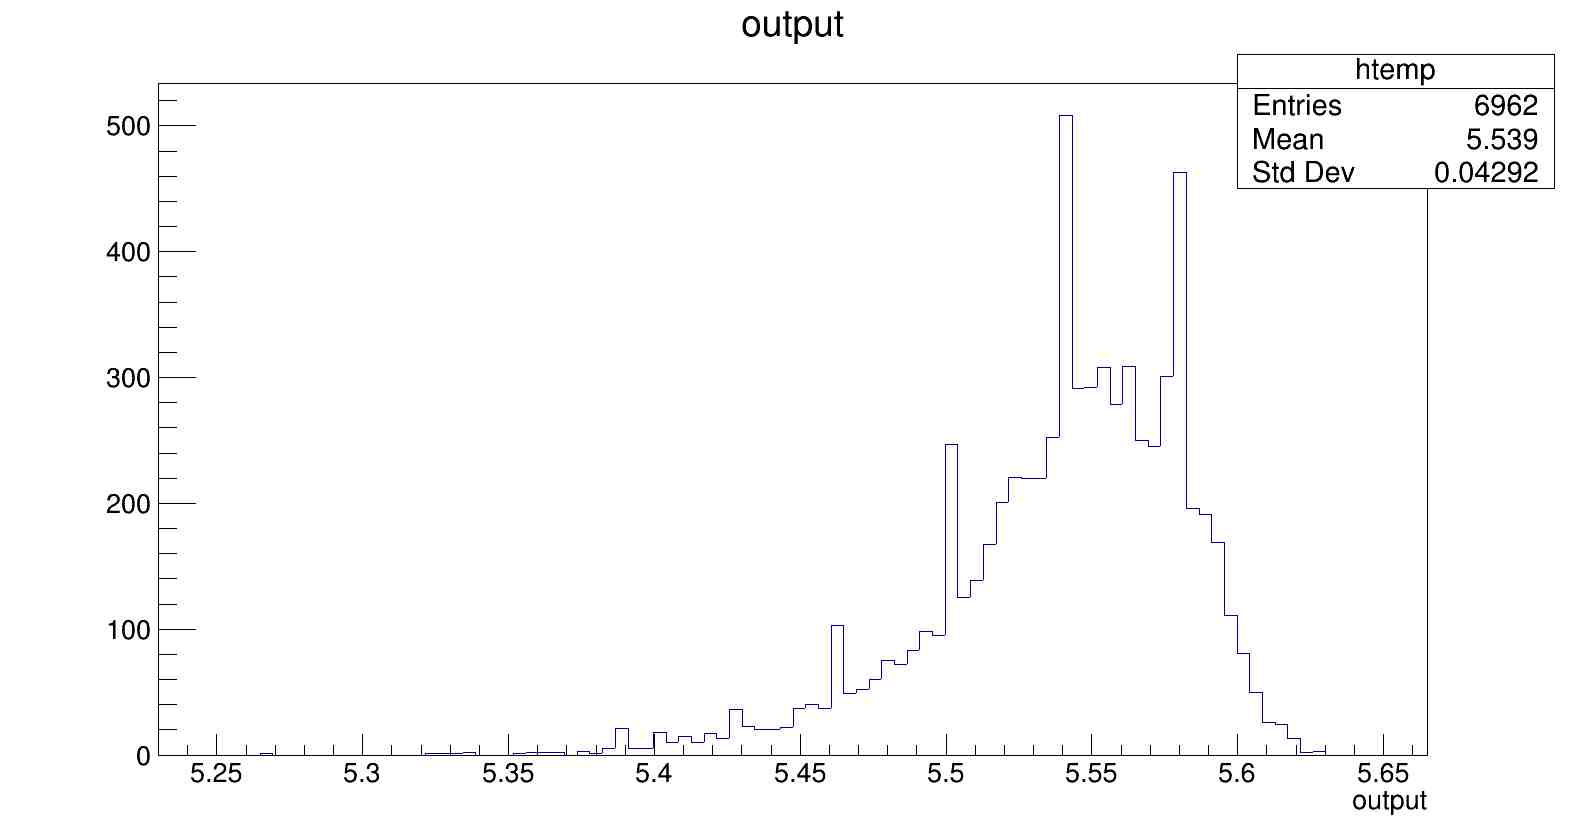
\includegraphics[width=0.75\linewidth]{figures/prediction.jpg}
    \caption{Prediction of 1 epoch without dropout layer}
    \label{}
\end{figure}
Result of 20 epochs, with 1 dropout layer,
\begin{figure}[H]
    \centering
    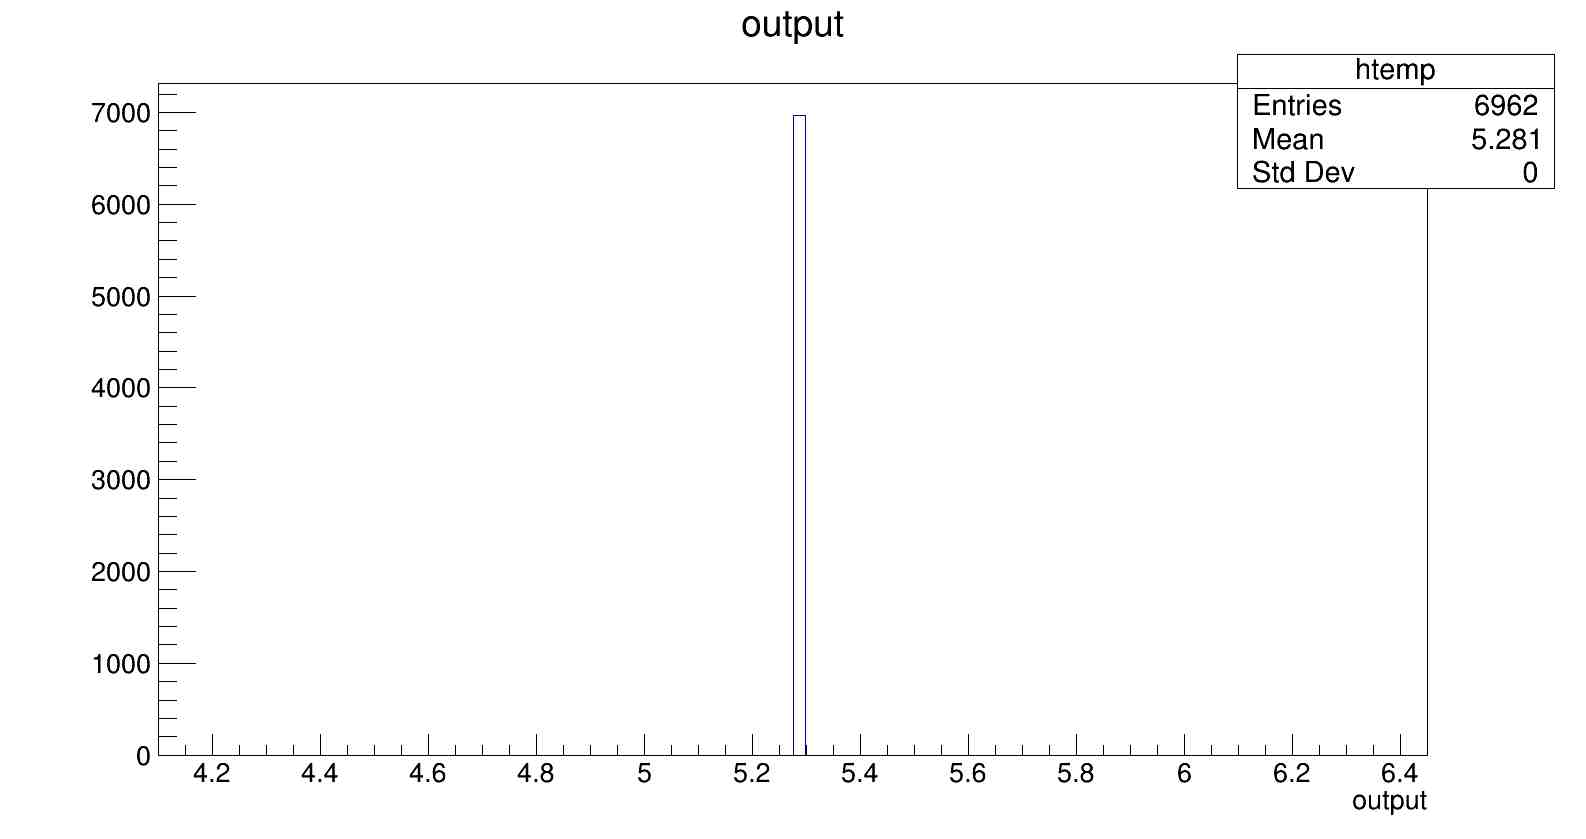
\includegraphics[width=0.75\linewidth]{figures/prediction20epochs.jpg}
    \caption{Prediction of 20 epochs with Dropout layer}
    \label{}
\end{figure}

\end{document}